\begin{visualexample}
\begin{center}
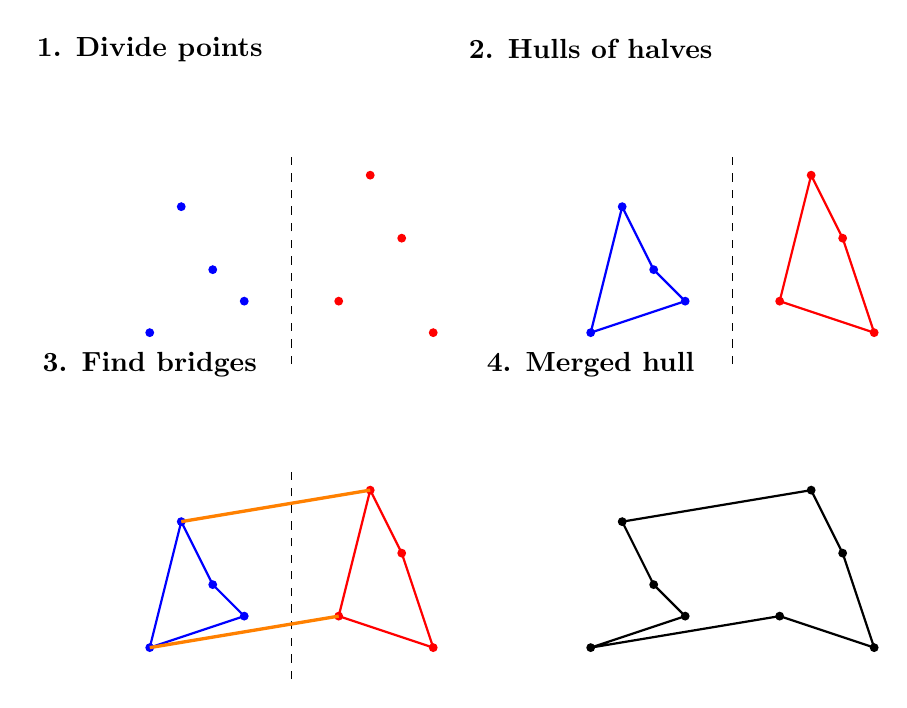
\begin{tikzpicture}[scale=0.8]
% Step 1: Points divided into left and right halves
\begin{scope}
\node at (0,4.5) {\textbf{1. Divide points}};
\fill[blue] (0,0) circle (2pt) (1,1) circle (2pt) (0.5,2) circle (2pt) (1.5,0.5) circle (2pt);
\fill[red] (3,0.5) circle (2pt) (4,1.5) circle (2pt) (3.5,2.5) circle (2pt) (4.5,0) circle (2pt);
\draw[dashed] (2.25,-0.5) -- (2.25,2.8);
\end{scope}

% Step 2: Convex hulls of each half
\begin{scope}[xshift=7cm]
\node at (0,4.5) {\textbf{2. Hulls of halves}};
\fill[blue] (0,0) circle (2pt) (1,1) circle (2pt) (0.5,2) circle (2pt) (1.5,0.5) circle (2pt);
\fill[red] (3,0.5) circle (2pt) (4,1.5) circle (2pt) (3.5,2.5) circle (2pt) (4.5,0) circle (2pt);
\draw[thick,blue] (0,0) -- (1.5,0.5) -- (1,1) -- (0.5,2) -- cycle;
\draw[thick,red] (3,0.5) -- (4.5,0) -- (4,1.5) -- (3.5,2.5) -- cycle;
\draw[dashed] (2.25,-0.5) -- (2.25,2.8);
\end{scope}

% Step 3: Upper and lower bridges highlighted
\begin{scope}[yshift=-5cm]
\node at (0,4.5) {\textbf{3. Find bridges}};
\fill[blue] (0,0) circle (2pt) (1,1) circle (2pt) (0.5,2) circle (2pt) (1.5,0.5) circle (2pt);
\fill[red] (3,0.5) circle (2pt) (4,1.5) circle (2pt) (3.5,2.5) circle (2pt) (4.5,0) circle (2pt);
\draw[thick,blue] (0,0) -- (1.5,0.5) -- (1,1) -- (0.5,2) -- cycle;
\draw[thick,red] (3,0.5) -- (4.5,0) -- (4,1.5) -- (3.5,2.5) -- cycle;
\draw[dashed] (2.25,-0.5) -- (2.25,2.8);
% Upper bridge
\draw[very thick,orange] (0.5,2) -- (3.5,2.5);
% Lower bridge
\draw[very thick,orange] (0,0) -- (3,0.5);
\end{scope}

% Step 4: Final merged hull
\begin{scope}[xshift=7cm, yshift=-5cm]
\node at (0,4.5) {\textbf{4. Merged hull}};
\fill (0,0) circle (2pt) (1,1) circle (2pt) (0.5,2) circle (2pt) (1.5,0.5) circle (2pt);
\fill (3,0.5) circle (2pt) (4,1.5) circle (2pt) (3.5,2.5) circle (2pt) (4.5,0) circle (2pt);
\draw[thick,black] (0,0) -- (1.5,0.5) -- (1,1) -- (0.5,2) -- (3.5,2.5) -- (4,1.5) -- (4.5,0) -- (3,0.5) -- cycle;
\end{scope}
\end{tikzpicture}
\end{center}
\end{visualexample}
